\documentclass[tikz,border=12pt]{standalone}
\usepackage[utf8]{inputenc}
\usepackage[T1]{fontenc}
\usepackage{lmodern}
\usepackage{amsmath}
\usepackage{chemformula}
\usetikzlibrary{arrows.meta,positioning,fit,backgrounds}

\definecolor{coseblue}{RGB}{0,70,140}
\definecolor{coseteal}{RGB}{22,138,128}
\definecolor{coseamber}{RGB}{217,119,6}
\definecolor{cosered}{RGB}{185,28,28}
\definecolor{slatebg}{RGB}{248,250,252}
\definecolor{slateborder}{RGB}{148,163,184}

\begin{document}
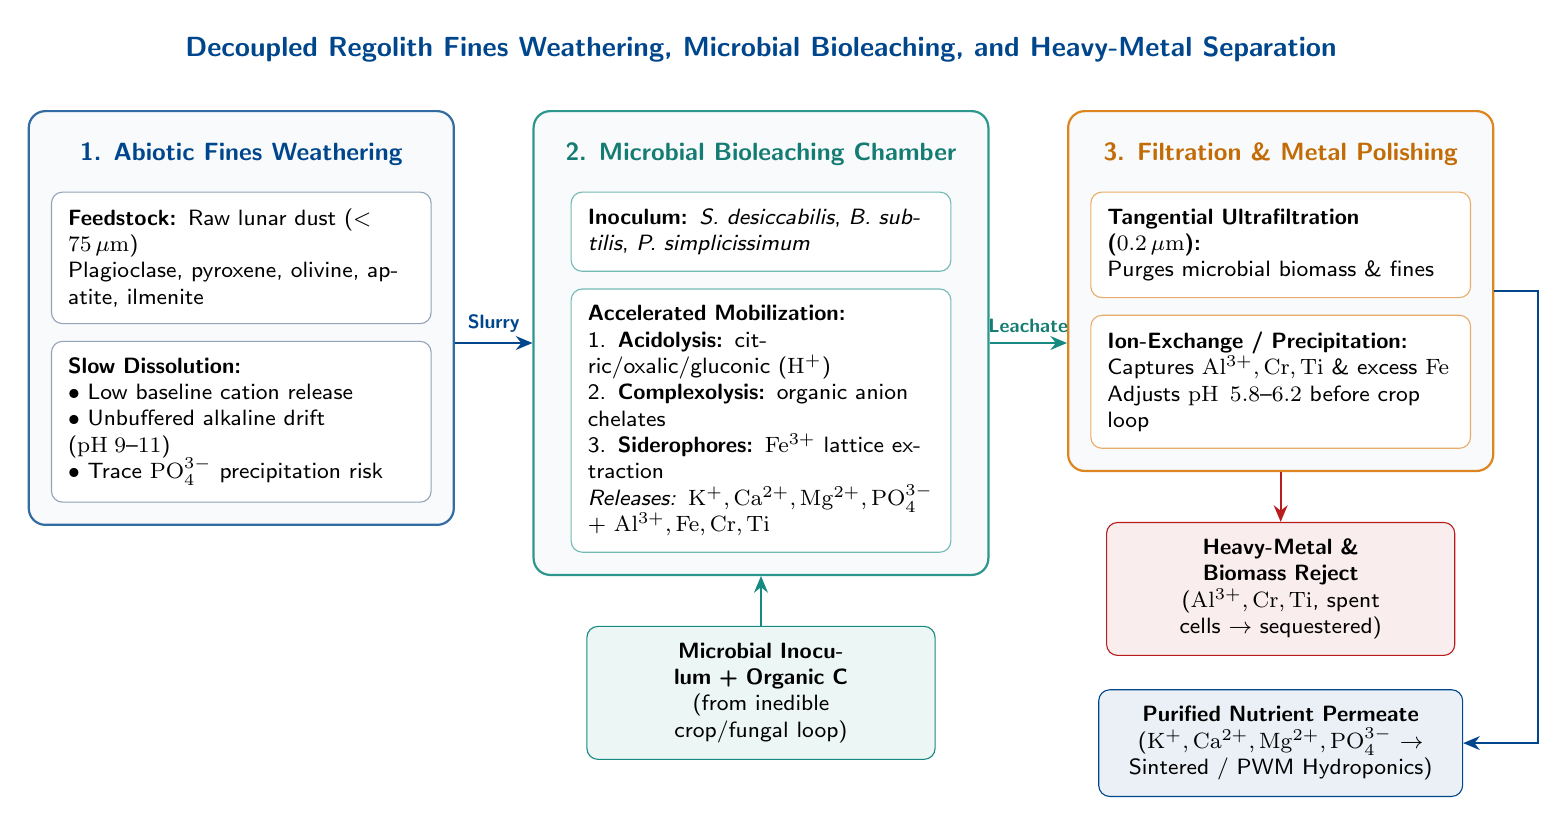
\begin{tikzpicture}[
    font=\sffamily\small,
    subbox/.style={
        draw=slateborder,
        rounded corners=4pt,
        fill=white,
        inner sep=6pt,
        align=left,
        font=\sffamily\footnotesize,
        text width=4.4cm
    },
    chambertitle/.style={
        font=\sffamily\bfseries\small,
        align=center
    },
    arrow/.style={
        -{Stealth[length=6pt,width=5pt]},
        thick,
        draw=coseblue
    },
    bioarrow/.style={
        -{Stealth[length=6pt,width=5pt]},
        thick,
        draw=coseteal
    },
    rejectarrow/.style={
        -{Stealth[length=6pt,width=5pt]},
        thick,
        draw=cosered
    }
]

% Stage 1 nodes
\node[chambertitle, text=coseblue] (t1) at (0, 2.8) {1. Abiotic Fines Weathering};
\node[subbox, below=6pt of t1] (s1a) {
    \textbf{Feedstock:} Raw lunar dust ($<75\,\mu\mathrm{m}$)\\
    Plagioclase, pyroxene, olivine, apatite, ilmenite
};
\node[subbox, below=6pt of s1a] (s1b) {
    \textbf{Slow Dissolution:}\\
    $\bullet$ Low baseline cation release\\
    $\bullet$ Unbuffered alkaline drift ($\mathrm{pH}\;9\text{--}11$)\\
    $\bullet$ Trace $\mathrm{PO_4^{3-}}$ precipitation risk
};

% Stage 2 nodes
\node[chambertitle, text=coseteal!90!black] (t2) at (6.6, 2.8) {2. Microbial Bioleaching Chamber};
\node[subbox, draw=coseteal!60, below=6pt of t2] (s2a) {
    \textbf{Inoculum:} \textit{S.\ desiccabilis}, \textit{B.\ subtilis}, \textit{P.\ simplicissimum}
};
\node[subbox, draw=coseteal!60, below=6pt of s2a] (s2b) {
    \textbf{Accelerated Mobilization:}\\
    1. \textbf{Acidolysis:} citric/oxalic/gluconic ($\mathrm{H}^+$)\\
    2. \textbf{Complexolysis:} organic anion chelates\\
    3. \textbf{Siderophores:} $\mathrm{Fe^{3+}}$ lattice extraction\\
    \textit{Releases:} $\mathrm{K^+, Ca^{2+}, Mg^{2+}, PO_4^{3-}}$ + $\mathrm{Al^{3+}, Fe, Cr, Ti}$
};

% Stage 3 nodes
\node[chambertitle, text=coseamber!90!black] (t3) at (13.2, 2.8) {3. Filtration \& Metal Polishing};
\node[subbox, draw=coseamber!60, below=6pt of t3] (s3a) {
    \textbf{Tangential Ultrafiltration ($0.2\,\mu\mathrm{m}$):}\\
    Purges microbial biomass \& fines
};
\node[subbox, draw=coseamber!60, below=6pt of s3a] (s3b) {
    \textbf{Ion-Exchange / Precipitation:}\\
    Captures $\mathrm{Al^{3+}, Cr, Ti}$ \& excess $\mathrm{Fe}$\\
    Adjusts $\mathrm{pH}\;5.8\text{--}6.2$ before crop loop
};

% Outer chamber frames fitted cleanly around contents
\begin{scope}[on background layer]
    \node[draw=coseblue!80, thick, rounded corners=6pt, fill=slatebg, inner sep=8pt, fit=(t1)(s1a)(s1b)] (c1) {};
    \node[draw=coseteal!90, thick, rounded corners=6pt, fill=slatebg, inner sep=8pt, fit=(t2)(s2a)(s2b)] (c2) {};
    \node[draw=coseamber!90, thick, rounded corners=6pt, fill=slatebg, inner sep=8pt, fit=(t3)(s3a)(s3b)] (c3) {};
\end{scope}

% Title Banner
\node[font=\sffamily\bfseries\normalsize, text=coseblue, above=14pt of c2] (title)
    {Decoupled Regolith Fines Weathering, Microbial Bioleaching, and Heavy-Metal Separation};

% Arrows between chambers (aligned horizontally)
\draw[arrow] (c1.east |- c2.west) -- node[above, font=\sffamily\scriptsize\bfseries, text=coseblue] {Slurry} (c2.west);
\draw[bioarrow] (c2.east) -- node[above, font=\sffamily\scriptsize\bfseries, text=coseteal!90!black] {Leachate} (c3.west |- c2.east);

% Bottom Inputs & Outputs
\node[subbox, draw=coseteal, fill=coseteal!8, text width=4.0cm, align=center, below=18pt of c2] (microbe_in) {
    \textbf{Microbial Inoculum + Organic C}\\
    (from inedible crop/fungal loop)
};
\draw[bioarrow] (microbe_in.north) -- (c2.south);

\node[subbox, draw=cosered, fill=cosered!8, text width=4.0cm, align=center, below=18pt of c3] (metal_out) {
    \textbf{Heavy-Metal \& Biomass Reject}\\
    ($\mathrm{Al^{3+}, Cr, Ti}$, spent cells $\to$ sequestered)
};
\draw[rejectarrow] (c3.south) -- (metal_out.north);

\node[subbox, draw=coseblue, fill=coseblue!8, text width=4.2cm, align=center, below=12pt of metal_out] (crop_out) {
    \textbf{Purified Nutrient Permeate}\\
    ($\mathrm{K^+, Ca^{2+}, Mg^{2+}, PO_4^{3-}}$ $\to$ Sintered / PWM Hydroponics)
};
\draw[arrow] (c3.east) -- ++(0.55, 0) |- (crop_out.east);

\end{tikzpicture}
\end{document}
